
\section{NDP}


\Cola{Neighbor Discovery Protocol (NDP) }is a protocol that solves a some problems
related to the interaction between nodes \cola{attached to the same link}. Some
of these problems inlcude:

\begin{itemize}
\item Router Discovery: \colz{how to find routers on the link.}
\item Prefix Discovery: \colz{how to find the addresses of other nodes on the
    link.(Nodes uses prefixes to distinguish destinations that reside on-link
    from those only reachable through a router (these are usually public IPs).)}
\item Parameter Discovery: \colz{how to find link parameters such as MTU.}
\item Address Autoconfiguration: \colz{how to assign addresses to nodes.}
\item ...and more
\end{itemize}

NDP defines five different ICMP packet types as shown in \cref{fig:dnp-5kinds}.

\begin{figure}
  \centering
  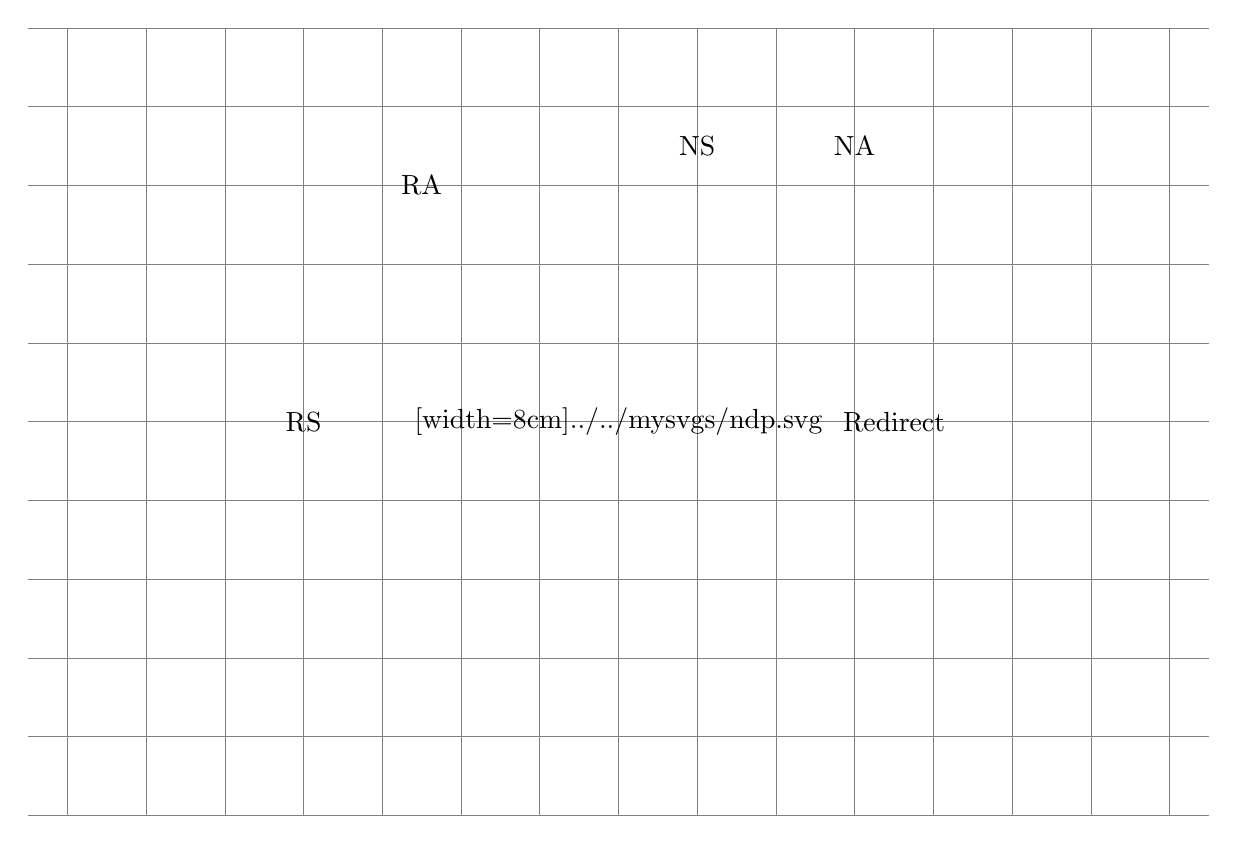
\begin{tikzpicture}
    \draw[step=1cm,help lines,] (-7.5cm,-5cm) grid +(15cm,10cm);
    \node at (0,0) {
    \includesvg[width=8cm]{../../mysvgs/ndp.svg}
    };

    \draw (-4cm,0) node {RS}
          (-2.5cm,3cm) node {RA}
          (1cm,3.5cm) node {NS}
          (3cm,3.5cm) node {NA}
          (3.5cm,0cm) node {Redirect}
    ;
    
  \end{tikzpicture}
  \caption{Five kinds of ICMP defined by NDP}
  \label{fig:dnp-5kinds}
\end{figure}

The 5 steps are shown in \cref{fig:dnp-step12,fig:dnp-step34,fig:dnp-step5}.

\dSay{
  What's contained in RA ?
}

\cSay{
  \colz{

    RA contains a lot of information. For example, it contains a \cola{list of
      prefixes} used for \colZ{on-link determination} and/or \colZ{autonomous
      address configuration};flags associated with the prefixes specify the
    \cola{intended uses of a particular prefix}.

    Hosts use the advertised on-link prefixes to build and maintain a list that
    is used in deciding when a packet's destination is on-link or beyond a
    router.

  }
}

\dSay{
  Do all traffic on the same link go through the router ?
}

\cSay{ \colz{ No. If the destination is on-link, then it is not covered by any
    advertised on- link prefix.

    In such cases, a router can send a \colZt{Redirect} informing
    the sender that the destination is a neighbor.   

    As a result, the traffic will be sent directly to the
    destination.
  }
}

\dSay{
  So when to use DHCPv6 and when to use autonomous (stateless) address configuration ?
}

\cSay{
  \colz{
    There's a flag in RA that indicates whether or not to use DHCPv6.
  }
}

\begin{figure}
  \centering
 \begin{tikzpicture}
  \draw[step=1cm,help lines,] (-7.5cm,-5cm) grid +(15cm,10cm);
  \tikzstyle{ndp-dialog}= [text width=7cm, fill=gray!10]
  \begin{scope}

    \node[below right, ndp-dialog] at (-7cm,5cm){
      \coli{Step 1: \texttt{Router Solicitation (RS)}:}
      {\color{gray}\small
        When an interface becomes enabled,
        hosts may send a \texttt{Router Solicitation} that request routers to
        generate \texttt{Router Advertisement} messages immediately.
        
      }
    };
    
    \node[above right, ndp-dialog] at (-4cm,-4cm){
      \colii{Step 2: \texttt{Router Advertisement(RA)}:}
      \colz{\small
        Routers advertise their presence and many parameters periodically and in
        response to a \texttt{Router Solicitation} message. (\emoji{parrot}: Oh,
        so it's like heartbeat. \emoji{turtle} : Yeah, kinda.) 
      }
    };
    
    \fill (3cm,0) circle (0pt)
    node {
      \includesvg[width=8cm]{../../mysvgs/ndp5.svg}
    };

    \coordinate (newcomer) at (-1cm,0);
    \coordinate (router) at (4cm,0);

    \leftDialogBoxColored[3cm]{newcomer}{
        1. Who's the router?
    }{\mycoli}

    \rightDialogBoxColored[2cm]{router}{
        2. Me
    }{\mycolii}
  \end{scope}
\end{tikzpicture}
  \caption{Step 1 and 2 of NDP}
  \label{fig:dnp-step12}
\end{figure}

\begin{figure}
  \centering
 \begin{tikzpicture}
  \draw[step=1cm,help lines,] (-7.5cm,-5cm) grid +(15cm,10cm);
  \tikzstyle{ndp-dialog}= [text width=7cm, fill=gray!10]
  \begin{scope}

    \node[below right, ndp-dialog] at (-7cm,5cm){
      \coliii{Step 3: \texttt{Neighbor Solicitation (NS)}:}
      {\color{gray}\small
        Sent by a node to
        \begin{enumerate}
        \item verify that a neighbor is still up.
        \item determine the link-layer address
        \end{enumerate}
        This is also used for \colZ{Duplicate Address Detection}
      }
    };

    \node[above right, ndp-dialog] at (-4cm,-4cm){
      \coliv{Step 4: \texttt{Neighbor Advertisement (NA)}:}
      \colz{\small
        A response to a \texttt{Neighbor Solicitation} message.
      }
    };
    
    \fill (3cm,0) circle (0pt)
    node {
      \includesvg[width=8cm]{../../mysvgs/ndp5.svg}
    };

    \coordinate (newcomer) at (-1cm,0);
    \coordinate (router) at (4cm,0);

    \coordinate (n1) at (1.6cm,3.6cm);
    \coordinate (n2) at (6cm,3.4cm);
    \coordinate (n3) at (6cm,-2.3cm);

    \leftDialogBoxColored[4cm]{newcomer}{
      3. Who's in ? \newline
      \small
      \colz{Okay..then I can't use these addresses.
      }
    }{\mycoliii}

    \foreach \i in {1,2,3}{
      \topDialogBoxColored[2cm]{n\i}{
        4. Me \texttt{fe80::\i}
      }{\mycoliv}
    }

  \end{scope}
\end{tikzpicture}
  \caption{Step 3 and 4 of NDP}
  \label{fig:dnp-step34}
\end{figure}

\begin{figure}
  \centering
 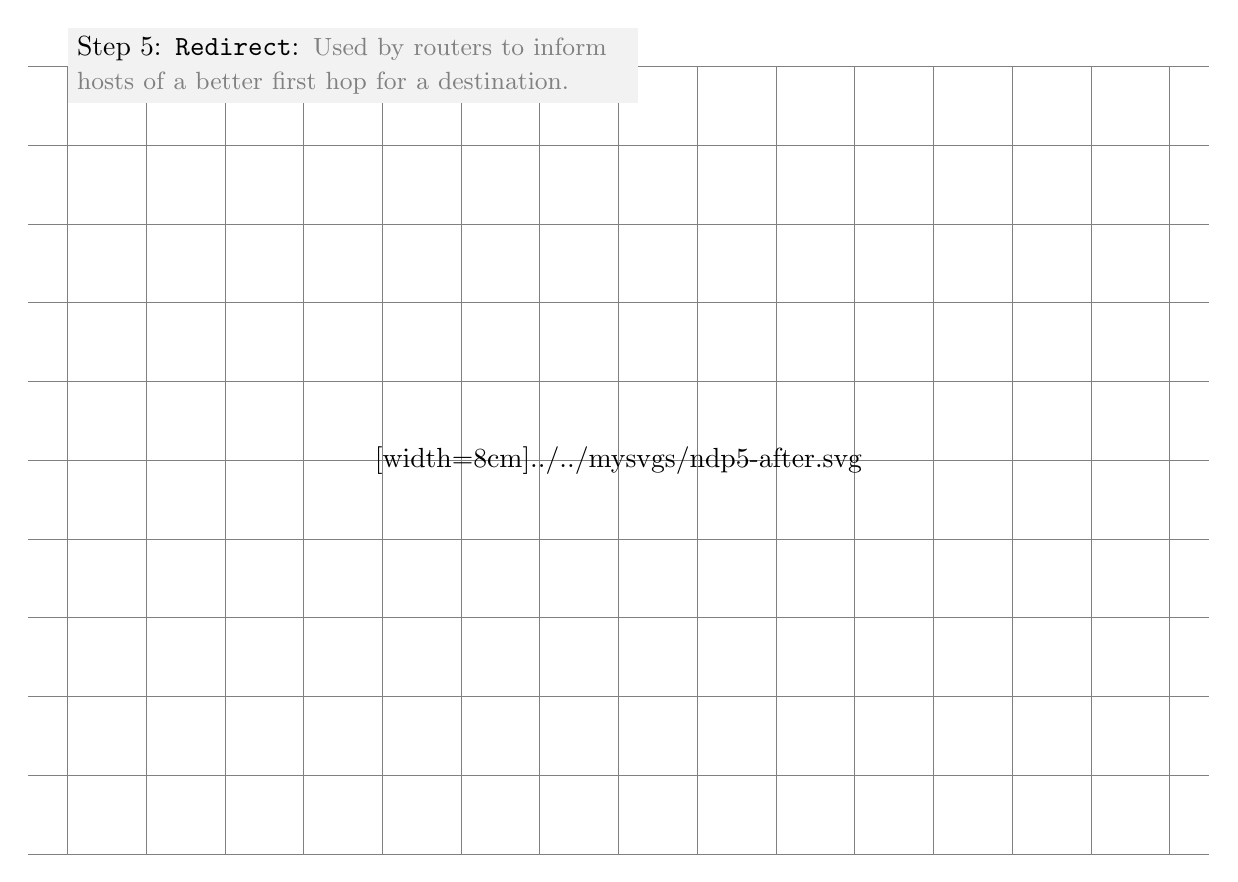
\begin{tikzpicture}
  \draw[step=1cm,help lines,] (-7.5cm,-5cm) grid +(15cm,10cm);
  \tikzstyle{ndp-dialog}= [text width=7cm, fill=gray!10]
  \begin{scope}

    \node[below right, ndp-dialog] at (-7cm,5.5cm){
      \colv{Step 5: \texttt{Redirect}:}
      {\color{gray}\small
        Used by routers to inform hosts of a better first hop for a destination.
      }
    };

    \fill (0cm,0) circle (0pt)
    node {
      \includesvg[width=8cm]{../../mysvgs/ndp5-after.svg}
    };

    \coordinate (router) at (-.5cm,0);

    \leftDialogBoxColored[3cm]{router}{
      5. Hey, guys, here's a better first hop for \texttt{2001:db8::1},....
    }{\mycolv}
  \end{scope}
\end{tikzpicture}
  \caption{Step 5 of NDP}
  \label{fig:dnp-step5}
\end{figure}

% flush all the floats
\clearpage